%This file is a child of preamble.Rnw in the style folder
%if you want to add stuff to the preamble go there to make
%your changes available to all childs

%<<setup-child, include = FALSE>>=
%library(knitr)
%set_parent("../style/preamble.Rnw")
%@

%<<size = "scriptsize", include=FALSE>>=
%source("code/functions.R")
%@


\documentclass[11pt,compress,t,notes=noshow]{beamer}

\usepackage[english]{babel}
\usepackage{dsfont}
\newcommand\bmmax{2}
\usepackage{bm}
\usepackage{bbm}
\usepackage{verbatim}
\usepackage{amsmath}
\usepackage{amsfonts}
\usepackage{csquotes}
\usepackage{multirow}
\usepackage{longtable}
\usepackage{enumerate}
\usepackage[absolute,overlay]{textpos}
\usepackage{psfrag}
\usepackage{algorithm}
\usepackage{algorithmicx}
\usepackage{algpseudocode}
\usepackage{eqnarray}
\usepackage{multimedia}
\usepackage{media9}
\usepackage{arydshln}
\usepackage{tabularx}
\usepackage{placeins}
\usepackage{tikz}
\usepackage{setspace}
\usepackage{wrapfig}
\usepackage{tcolorbox}
\usepackage[export]{adjustbox}
\usepackage{siunitx}
\usetikzlibrary{shapes,arrows,automata,positioning,calc}
\def\signed #1{{\leavevmode\unskip\nobreak\hfil\penalty50\hskip1em
  \hbox{}\nobreak\hfill #1%
  \parfillskip=0pt \finalhyphendemerits=0 \endgraf}}

\newsavebox\mybox
\newenvironment{aquote}[1]
  {\savebox\mybox{#1}\begin{quote}\openautoquote\hspace*{-.7ex}}
  {\unskip\closeautoquote\vspace*{1mm}\signed{\usebox\mybox}\end{quote}}
  
\tikzset{
  %Define standard arrow tip
  >=stealth',
  %Define style for boxes
  punkt/.style={
    rectangle,
    rounded corners,
    draw=black, very thick,
    text width=6.5em,
    minimum height=2em,
    text centered},
  % Define arrow style
  pil/.style={
    ->,
    thick,
    shorten <=2pt,
    shorten >=2pt,}
}
\usepackage{subfig}

%new environments

\newenvironment{vbframe}  %frame with breaks and verbatim
{
 \begin{frame}[containsverbatim,allowframebreaks]
}
{
\end{frame}
}

\newenvironment{vframe}  %frame with verbatim without breaks (to avoid numbering one slided frames)
{
 \begin{frame}[containsverbatim]
}
{
\end{frame}
}

\newenvironment{blocki}[1]   % itemize block
{
 \begin{block}{#1}\begin{itemize}
}
{
\end{itemize}\end{block}
}

\newenvironment{fragileframe}[2]{  %fragile frame with framebreaks
\begin{frame}[allowframebreaks, fragile, environment = fragileframe]
\frametitle{#1}
#2}
{\end{frame}}


\newcommand{\myframe}[2]{  %short for frame with framebreaks
\begin{frame}[allowframebreaks]
\frametitle{#1}
#2
\end{frame}}

\newcommand{\remark}[1]{
  \textbf{Remark:} #1
}

%%%%%%%%%%%%%%%%%%%%%%%%%%%%%%%%%%%%%%%%%%%%%%%%%%%%%%%%%%%%%%%%%%%%%%%%%%%%%%%

% basic latex stuff
\newcommand{\pkg}[1]{{\fontseries{b}\selectfont #1}} %fontstyle for R packages
\newcommand{\lz}{\vspace{0.5cm}} %vertical space
\newcommand{\dlz}{\vspace{1cm}} %double vertical space
\newcommand{\oneliner}[1] % Oneliner for important statements
{\begin{block}{}\begin{center}\begin{Large}#1\end{Large}\end{center}\end{block}}


%\usetheme{lmu-lecture}
\usepackage{../style/lmu-lecture}

\let\code=\texttt
\let\proglang=\textsf

\setkeys{Gin}{width=0.9\textwidth}


\title{Introduction to Machine Learning}
\author{Bernd Bischl}
\institute{Department of Statistics -- LMU Munich}
\date{Winter term 2021}

\setbeamertemplate{frametitle}{\expandafter\uppercase\expandafter\insertframetitle}

\begin{document}
\sloppy
\end{document}


\input{../latex-math/basic-math}
\input{../latex-math/basic-ml}
\input{../latex-math/ml-nn}

\begin{document} 
\lecturechapter{1}{Deep Learning- Introduction}
\lecture{Deep Learning - Introduction}


%%%%%%%%%%%%%%%%%%%%%%%%%%%%%%%%%%%%%%%%%%%%%%%%%%%%%%%%%%%%%%%%%%

\begin{frame} {What is Deep Learning}



\begin{center}
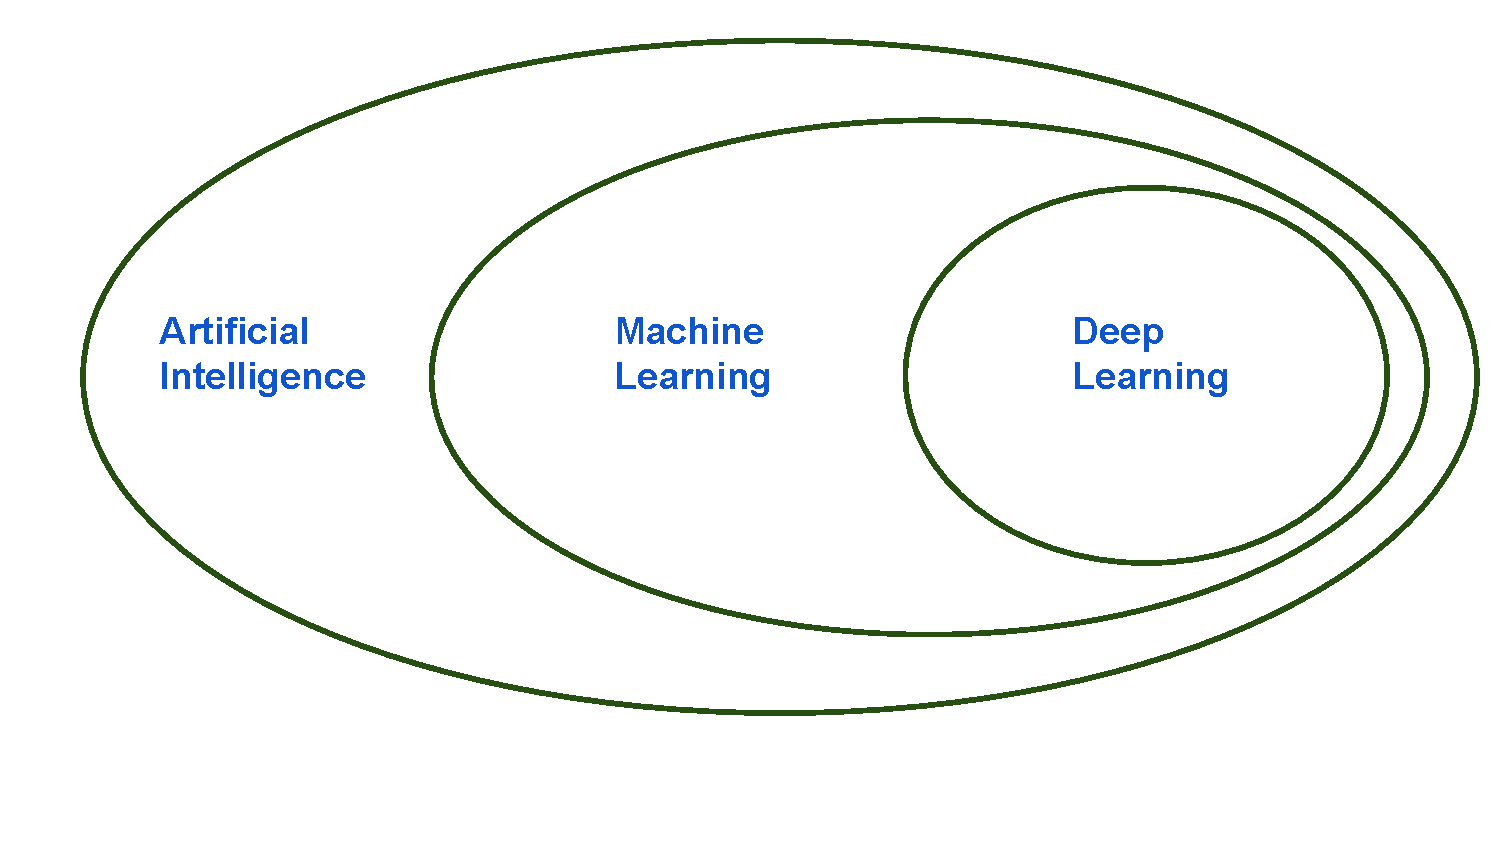
\includegraphics[width=0.95\textwidth]{plots/learning.pdf}
\end{center}

\vspace{-.5cm}
  \begin{itemize}
    \item Deep learning is the use of artificial neural networks to
construct models on large amounts of (unstructured) data.
    \end{itemize}
\end{frame}

%%%%%%%%%%%%%%%%%%%%%%%%%%%%%%%%%%%%%%%%%%%%%%%%%%%%%%%%%%%%%%%%%%

\begin{frame} {Deep Learning and Neural Networks}
\begin{itemize}
\item Deep learning and neural networks are mostly equivalent.
\vspace{.3cm}
\item Deep learning itself is not \textit{new}:
\begin{itemize}
\item Neural networks have been around since the 70s
\item \textit{Deep} neural networks, i.e., networks with multiple hidden layers, are not much younger.
\end{itemize}
\vspace{.3cm}
\item Why everybody is talking about deep learning now:
\begin{itemize}
\item Specialized, powerful hardware allows the training of huge neural networks that are able to push the state-of-the-art on extremely difficult problems.
\item Large amount of data is available.
\item Special network architectures for image/text data.
\item Better optimization and regularization strategies.
\end{itemize}
\end{itemize}
\end{frame}

%%%%%%%%%%%%%%%%%%%%%%%%%%%%%%%%%%%%%%%%%%%%%%%%%%%%%%%%%%%%%%%%%%
\begin{frame}{Image Classification with Neural Networks}

\begin{aquote}{Y. Bengio}
Machine learning algorithms, inspired by the brain, based on learning multiple levels of representation/abstraction.   
\end{aquote}

\begin{overlayarea}{\textwidth}{\textheight}
    \only<1>{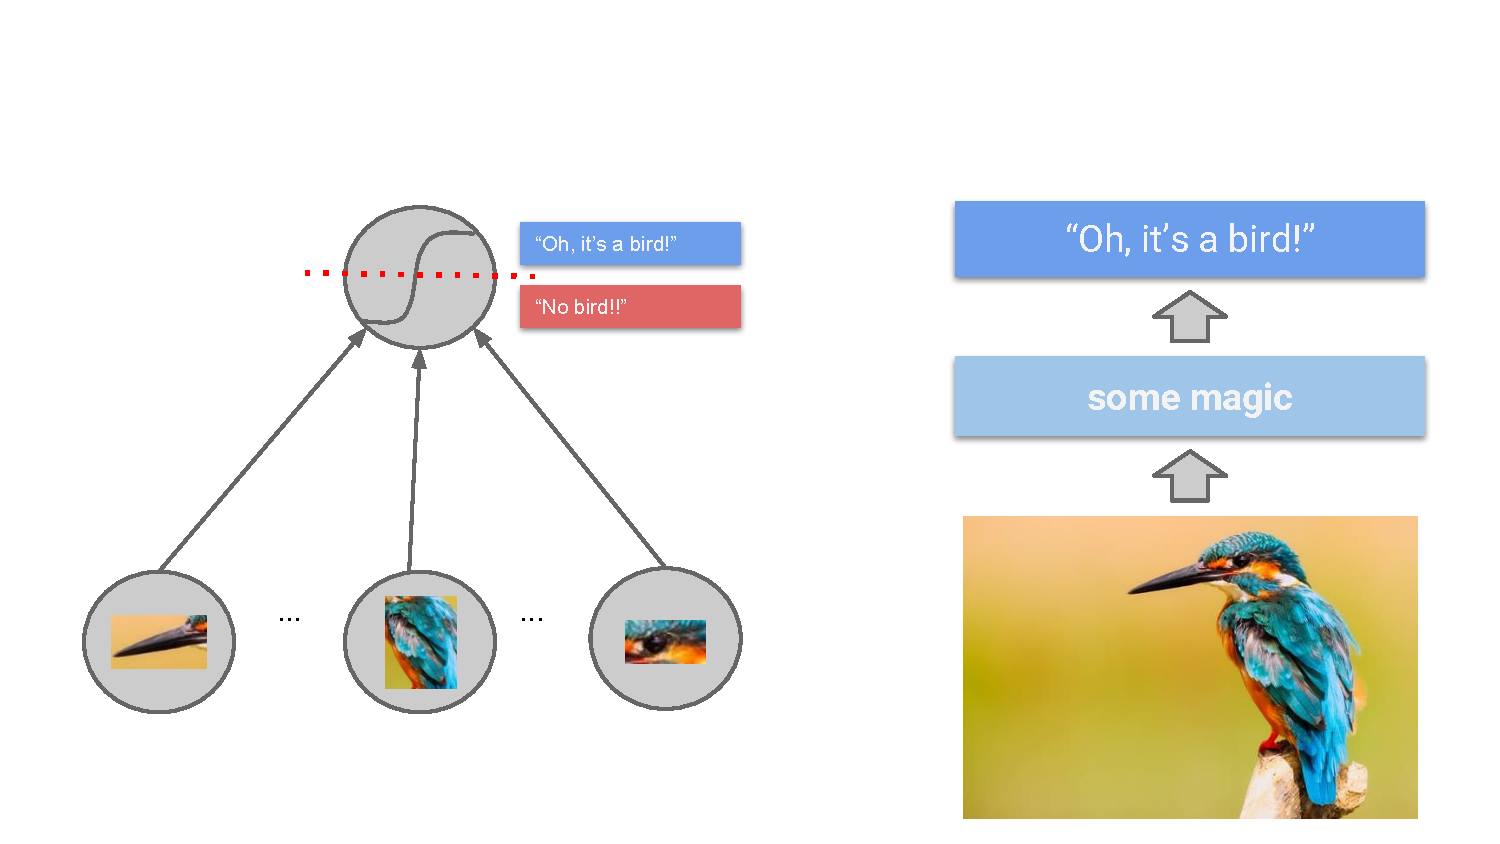
\includegraphics[width=\textwidth]{plots/bird1.pdf}}
    \only<2>{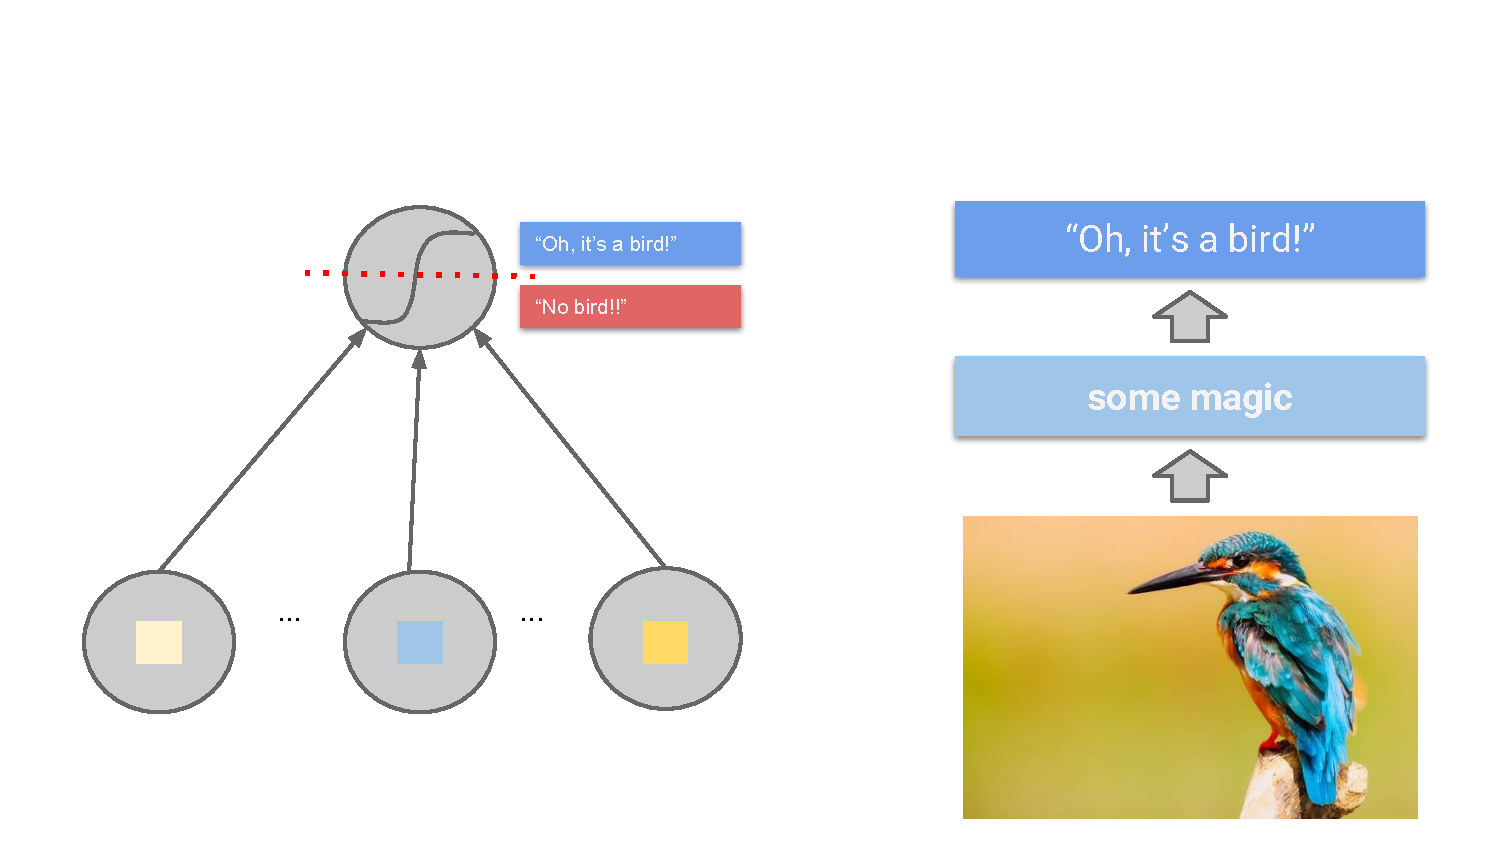
\includegraphics[width=\textwidth]{plots/bird2.pdf}}
    \only<3>{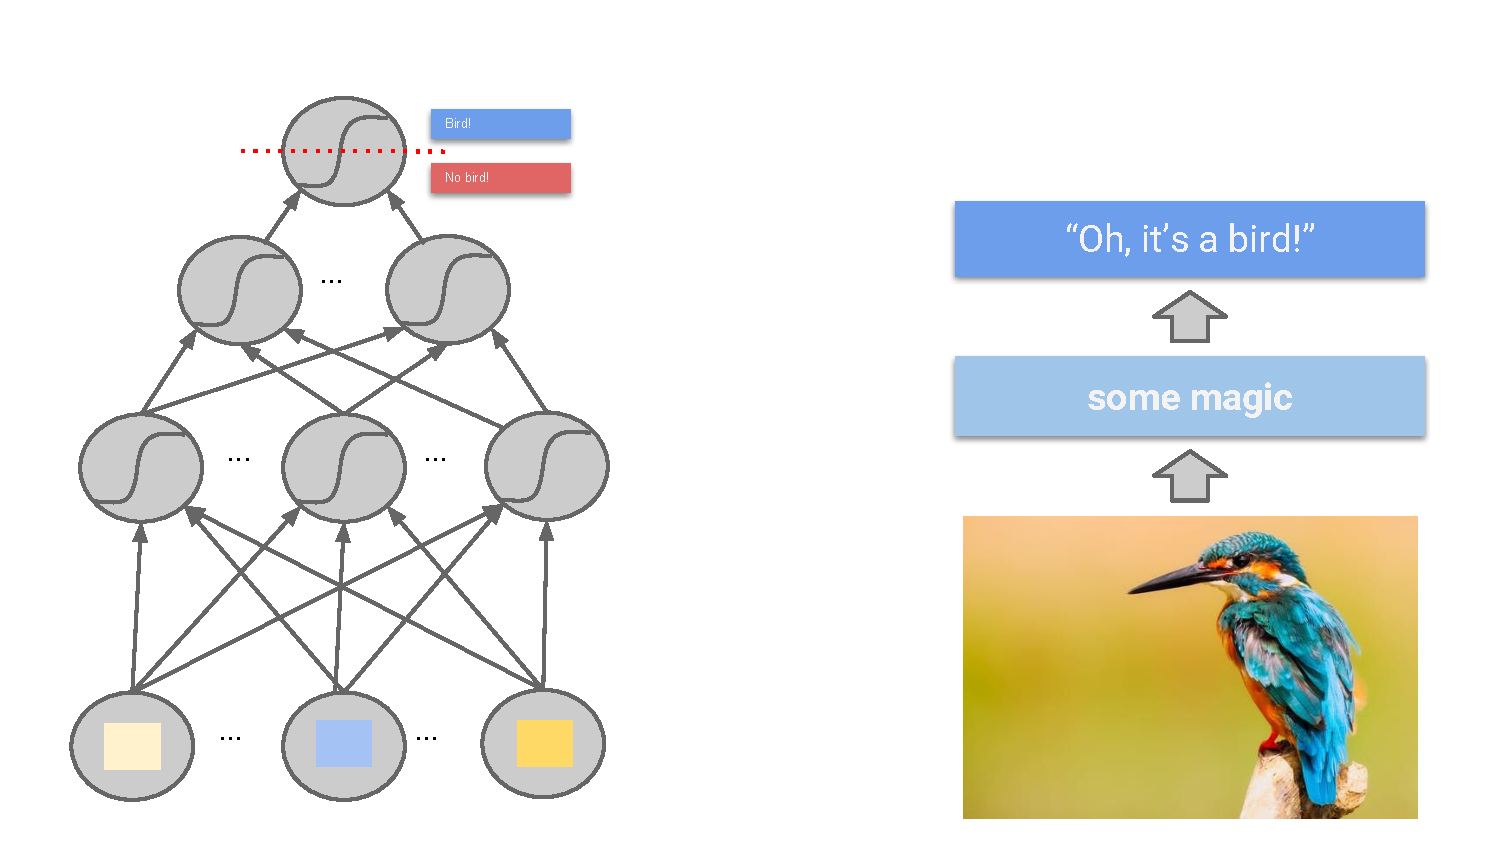
\includegraphics[width=\textwidth]{plots/bird3.pdf}}
    \only<4>{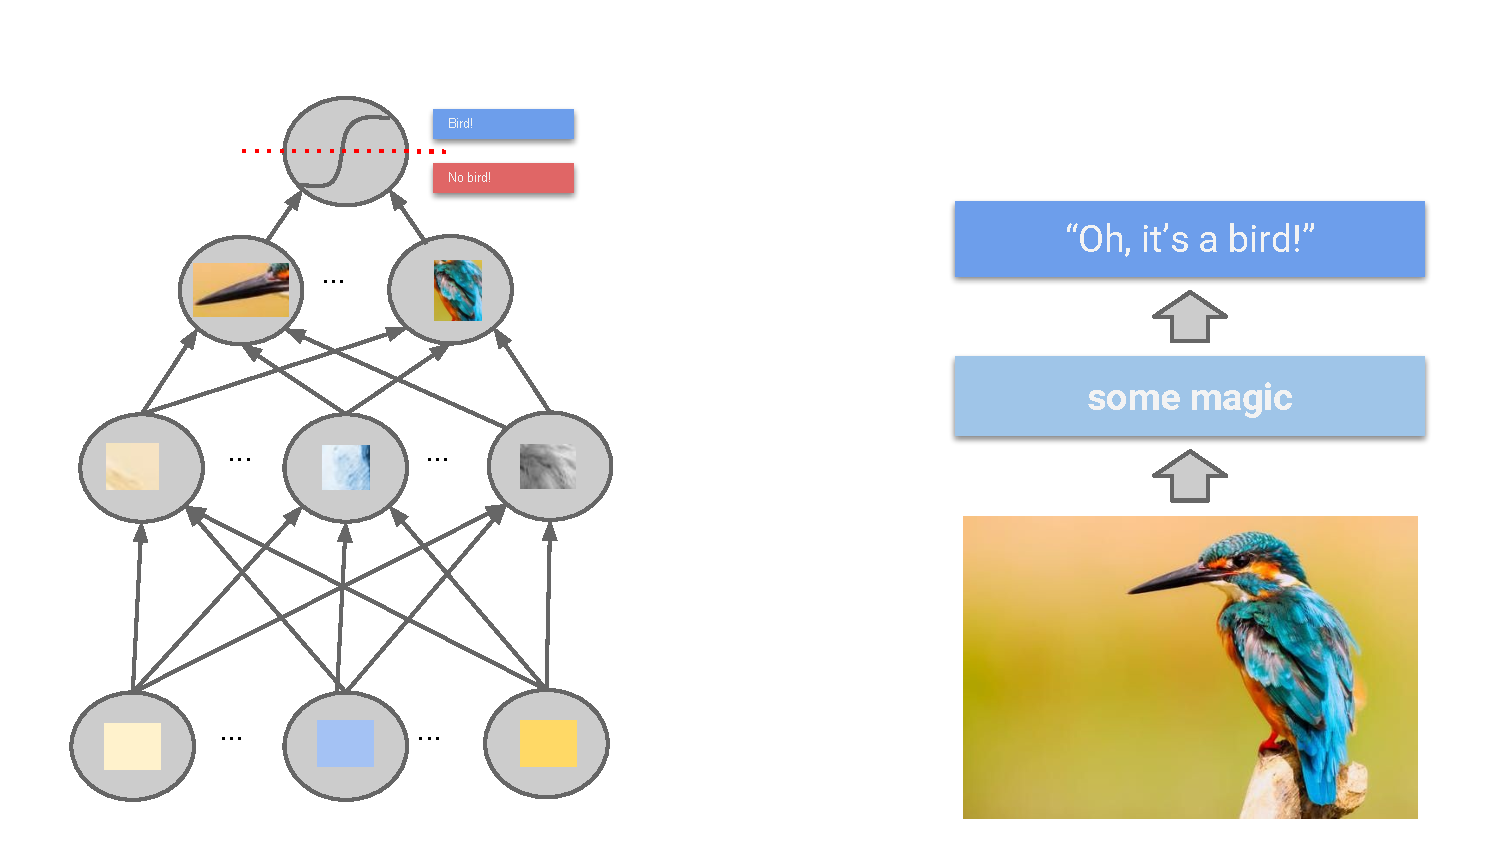
\includegraphics[width=\textwidth]{plots/bird4.pdf}}
\end{overlayarea}


\end{frame}

%%%%%%%%%%%%%%%%%%%%%%%%%%%%%%%%%%%%%%%%%%%%%%%%%%%%%%%%%%%%%%%%%%

\begin{frame} {Possible use-cases}


\textbf{Deep learning can be extremely valuable if the data has these properties:}
\vspace{.2cm}
\begin{itemize}
\item It is high dimensional.
\item Each single feature itself is not very informative but only a combination of them might be.
\item There is a large amount of training data.
\end{itemize}

\vspace{.7cm}

\textbf{This implies that for tabular data, deep learning is almost never the correct model choice.}
\vspace{.2cm}
\begin{itemize}
\item Models like random forests or gradient boosting will outperform deep learning most of the time.
\item One exception can be data with categorical features with many levels.
\end{itemize}

\end{frame}


%%%%%%%%%%%%%%%%%%%%%%%%%%%%%%%%%%%%%%%%%%%%%%%%%%%%%%%%%%%%%%%%%%

\begin{frame} {Possible use-case: Images}

\begin{itemize}
\item \textbf{High Dimensional}: A color image with $255 \times 255$ (3 Colors) pixels already has $195075$ features.
\vspace{.5cm}
\item \textbf{Informative}: A single pixel is not meaningful in itself.
\vspace{.5cm}
\item \textbf{Training Data}: Depending on applications huge amounts of data are available.
\end{itemize}
\vspace{1.5cm}
Architecture: \textbf{C}onvolutional \textbf{N}eural \textbf{N}etworks (CNN)
\end{frame}

%%%%%%%%%%%%%%%%%%%%%%%%%%%%%%%%%%%%%%%%%%%%%%%%%%%%%%%%%%%%%%%%%%

\begin{frame} {Possible use-case: Images}

\begin{figure}
\centering
\scalebox{.7}{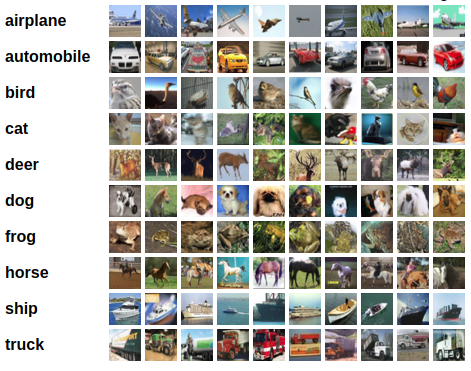
\includegraphics{plots/classification.png}}
\end{figure}

\textbf{Image classification} tries to predict a single label for each image (Alex Krizhevsky (2009))

CIFAR-10 is a well-known dataset used for image classification. It consists of $60,000$ $32x32$ color images containing one of $10$ object classes, with $6000$ images per class. 

\end{frame}

%%%%%%%%%%%%%%%%%%%%%%%%%%%%%%%%%%%%%%%%%%%%%%%%%%%%%%%%%%%%%%%%%%

\begin{frame} {Possible use-case: Images}

\begin{figure}
\centering
\scalebox{0.8}{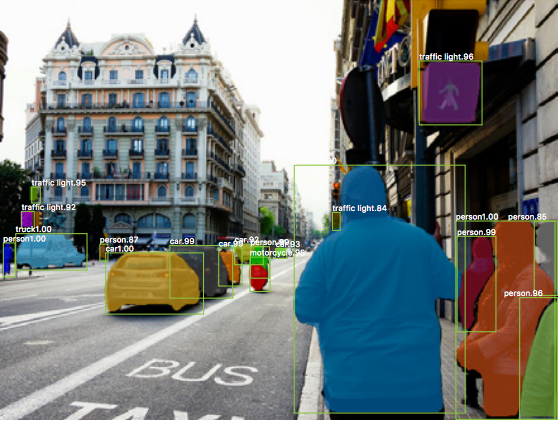
\includegraphics{plots/maskrcnn.png}}
\end{figure}
  
\textbf{Object Detection} (Kaiming He (2017))

Mask R-CNN is a general framework for instance segmentation, which efficiently detects objects in an image while simultaneously generating a high-quality segmentation mask for each instance.
\end{frame}

%%%%%%%%%%%%%%%%%%%%%%%%%%%%%%%%%%%%%%%%%%%%%%%%%%%%%%%%%%%%%%%%%%


\begin{frame} {Possible use-case: Images}

\begin{figure}
\centering
\scalebox{.8}{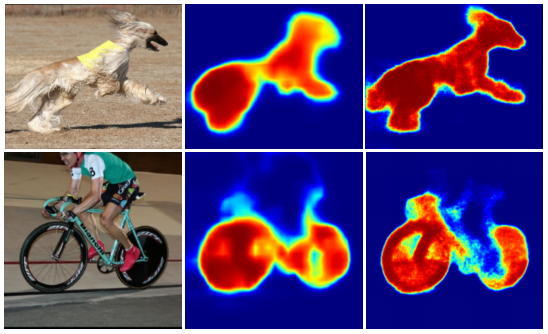
\includegraphics{plots/segmentation.png}}
\end{figure}
  
\textbf{Image segmentation} partitions the image into (multiple) segments (Hyeonwoo Noh (2015))

\end{frame}

%%%%%%%%%%%%%%%%%%%%%%%%%%%%%%%%%%%%%%%%%%%%%%%%%%%%%%%%%%%%%%%%%%


\begin{frame} {Possible use-case: Text}


\begin{itemize}
\item \textbf{High Dimensional}: Each word can be a single feature (~300000 words in the German language).
\vspace{.5cm}
\item \textbf{Informative}: A single word does not provide much context.
\vspace{.5cm}
\item \textbf{Training Data}: Huge amounts of text data available.
\end{itemize}
\vspace{1.5cm}
Architecture: \textbf{R}ecurrent \textbf{N}eural \textbf{N}etworks (RNN)

\end{frame}

%%%%%%%%%%%%%%%%%%%%%%%%%%%%%%%%%%%%%%%%%%%%%%%%%%%%%%%%%%%%%%%%%%

\begin{frame} {Possible use-case: Text}

Applications:
\vspace{.7cm}
\begin{itemize}
\item \textbf{N}atural \textbf{L}anguage \textbf{P}rocessing, e.g.,
\begin{itemize}
\item Sentiment Analysis
\vspace{.3cm}
\item Email Classification
\vspace{.3cm}
\item Chat-bots
\vspace{.3cm}
\item $...$
\end{itemize}
\vspace{.7cm}
\item Modeling Sequential Data (Time-Series, Speech)
\end{itemize}

\end{frame}
%%%%%%%%%%%%%%%%%%%%%%%%%%%%%%%%%%%%%%%%%%%%%%%%%%%%%%%%%%%%%%%%%%

\begin{frame} {Possible use-case: Text}

  \begin{figure}
    \centering
      \scalebox{.9}{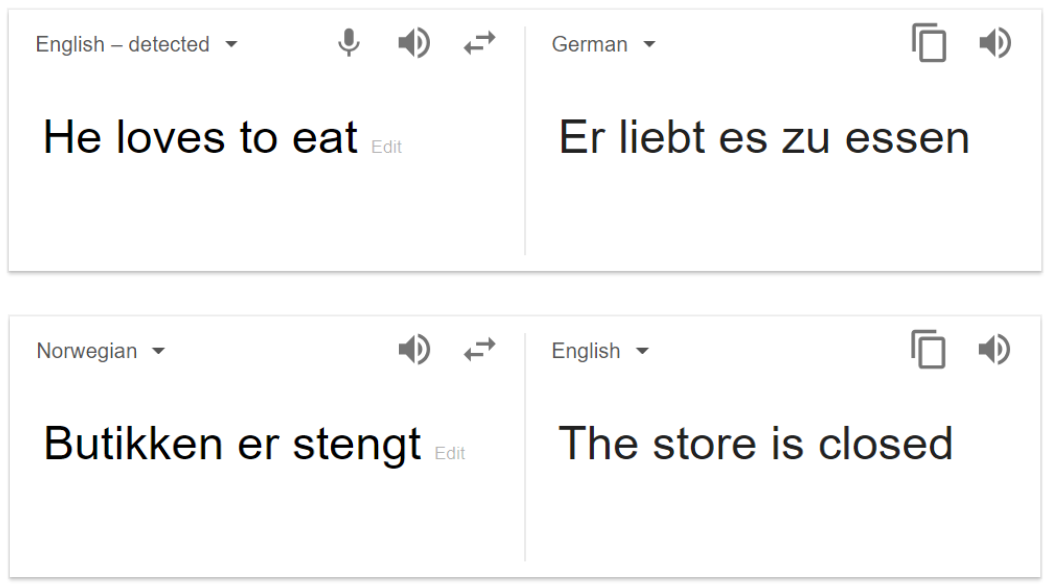
\includegraphics{plots/nmt.png}}
  \end{figure}
  
\textbf{Machine Translation} (e.g. google translate) 

Neural machine translation exploits neural networks to predict the likelihood of a sequence of words, typically modeling entire sentences in a single integrated model.
\end{frame}

%%%%%%%%%%%%%%%%%%%%%%%%%%%%%%%%%%%%%%%%%%%%%%%%%%%%%%%%%%%%%%%%%%
\begin{frame} {Applications of Deep Learning: Speech}

  \begin{figure}
    \centering
      \scalebox{.9}{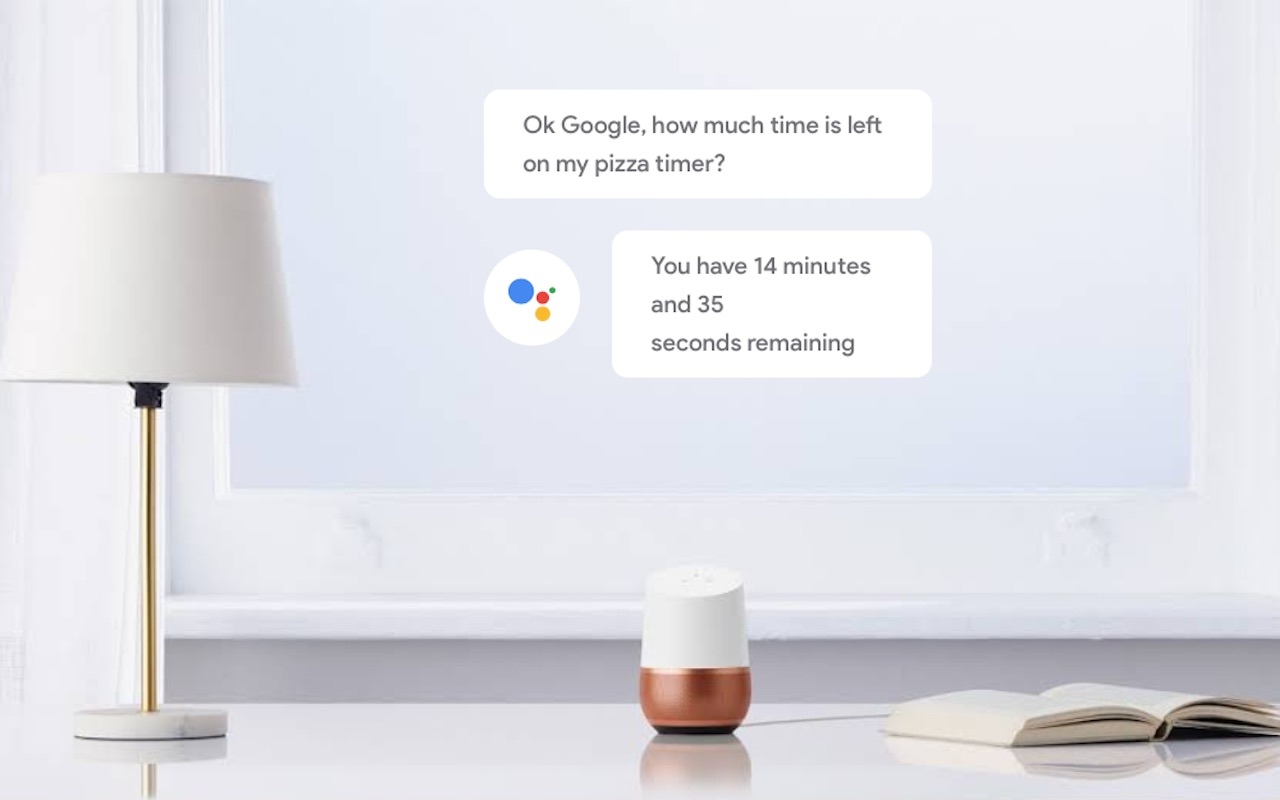
\includegraphics{plots/speech_goog.jpg}}
  \end{figure}
  
\textbf{Speech Recognition and Generation} (e.g. google assistant)

Neural network extracts features from audio data in order to classify emotions in speech.

\end{frame}

%%%%%%%%%%%%%%%%%%%%%%%%%%%%%%%%%%%%%%%%%%%%%%%%%%%%%%%%%%%%%%%%%%
\endlecture

\end{document}